\documentclass[11pt]{article}
\usepackage[margin=1in]{geometry}
\usepackage{amsmath}
\usepackage{booktabs}
\usepackage{graphicx}
\usepackage{tabularx}
\usepackage{caption}
\usepackage{microtype}
\usepackage{xcolor}
\usepackage{url}
\usepackage[hidelinks]{hyperref}
\usepackage{enumitem}
\setlist{topsep=2pt,itemsep=2pt}
\urlstyle{tt}
\newcommand{\modelonly}{\textsc{model-only}}
\newcommand{\code}[1]{\texttt{\small #1}}

\title{\textbf{Resilient Emergency MANETs for Wilderness Safety}\\[4pt]
\large Directed Study Final Report}
\author{Ethan Doherty\\\small Directed Study (CS 5976) --- Advisors: Prof.~Guevara and Prof.~S.~Basagni}
\date{July 26, 2026\\[3pt]
\small Code, data, and all cited artifacts:
\url{https://github.com/edoherty2017/resilient-emergency-manets-final}}

\begin{document}
\maketitle

\begin{abstract}
\noindent This directed study delivered a purpose-built, two-engine
(Python/Rust) discrete-event simulation framework for year-scale energy and
reliability analysis of a Meshtastic-style wilderness mesh --- cross-validated on a shared micro-scenario between independently written engines (statewide parity pending), byte-reproducible, and released with hash-locked inputs --- together with a Longley--Rice ITM terrain planning
layer, a preregistration-grade field methodology, and a field acquisition system proven receiver-side end-to-end in the field. Its principal \modelonly{} insight:
network survivability is governed by the idle-listening/duty-cycling policy,
not the routing algorithm --- five distinct always-on routing modes differ by
$<0.3\%$ in annual battery depletions while duty policies move depletions by
${\approx}5.5$--$24\times$, at a quantified cost in delivery ratio and SOS
latency. The empirical program was adjusted in flight, with every adjustment
registered before collection: Trial~1 served as a systems shakedown, and
Trial~2 ran as a field campaign of four field days plus a fifth registered
siting (2026-07-18 to 2026-07-26), re-planned after the beacon node's
hardware failed, ending with an operationally successful receiver-only field
day that produced two quantified findings substantiating the necessity of the controlled-beacon design (transmit-opportunity starvation; hop ambiguity). The planned
calibration dataset was not obtained --- 0 of the ${\geq}2{,}500$ planned points --- and its acquisition is a small, fully specified next step: a
${\approx}\$25$ replacement beacon and one two-radio field day under the
already-frozen protocol.
\end{abstract}

\section{Original objectives and what changed}\label{sec:objectives}

The original plan (preserved unedited in \path{docs/execution-roadmap-weekly.md})
had five success criteria:

\begin{table}[h]
\small
\begin{tabularx}{\textwidth}{@{}p{4.2cm}X@{}}
\toprule
\textbf{Original objective} & \textbf{Outcome} \\
\midrule
Architecture and design documentation & Delivered (\path{docs/system-architecture.md} and related). \\
${\geq}2{,}500$ empirical field points & \textbf{Not met --- 0 calibration-grade points.} Trial~1 produced 0 calibration-eligible observations (\S\ref{sec:trial1}); Trial~2's four field days (plus a fifth registered siting, \S\ref{sec:trial2}) were ended by beacon hardware failure before any controlled link ran. A per-stratum replacement metric (${\geq}40$ scheduled opportunities per primary stratum) is a \emph{proposed} amendment awaiting advisor review. \\
AIRMap calibration files & \textbf{Not produced} --- blocked on controlled data; the gated pipeline that will produce them is built and tested. \\
10--15 page validation report (RMSE/MAE, heatmaps, failure matrix) & \textbf{Deferred, not abandoned.} All builder tooling exists; producible immediately after a two-radio field day (\S\ref{sec:future}). \\
Large-scale simulation as optional appendix & \textbf{Inverted:} the simulation became the central completed contribution (\S\ref{sec:sim}--\S\ref{sec:findings}). \\
\bottomrule
\end{tabularx}
\end{table}

Amendments and standing: the RSRP$\to$ESP substitution is drafted but
unsigned (disclosed, not assumed); the ${\geq}40$-opportunity rule is
proposed, not approved; the study area is New Hampshire only; the planned
Tuckerman/Huntington campaigns were replaced by the Ammonoosuc--Jewell system
and then, in the field week, by the Moosilauke~$\to$ Monadnock~$\to$ Pack
Monadnock sequence (\S\ref{sec:trial2}, each step registered before
collection). Radio operation across all field days used stock FCC-certified
consumer hardware in its as-marketed configuration (\S\ref{sec:packday});
production-deployment authorization deferred (\S\ref{sec:limits}). The defensible scientific claim narrowed from
``a validated emergency-network design'' to ``an uncalibrated planning and
sensitivity framework plus a field-acquisition system awaiting controlled
empirical validation.''

\section{Simulator architecture}\label{sec:sim}

Two independent implementations of one model: \code{scripts/mesh\_sim.py}
(SimPy reference engine, detailed event traces) and \code{fastsim/} (Rust;
summary-only engine for long horizons and multi-seed sweeps; nine shared
modes --- flood, min\_hop, etx, energy\_aware, lb\_energy, duty\_sync,
duty\_adaptive, rotate\_lb, selective\_duty; validated inputs; atomic output;
deterministic tie-breaking). Randomness is keyed per phenomenon and entity,
so workloads are comparable across algorithms and a congested MAC cannot
alter the offered load.

\paragraph{Propagation/reception.} Received power $=$ 26.30\,dBm reference
(24.15\,dBm TX EIRP $+$ 2.15\,dBi RX antenna gain $+$ assumed 0\,dB feed loss
--- the reference is \emph{not} EIRP) minus a link-specific median loss, plus
Gauss--Markov slow shadowing ($\sigma = 8$\,dB, 30\,s coherence) and a 2\,dB
per-packet fast term. Median loss: fixed$\leftrightarrow$fixed links use
precomputed Longley--Rice ITM q50 over USGS 3DEP terrain;
mobile$\leftrightarrow$fixed uses time-interpolated route-loss tables;
mobile$\leftrightarrow$mobile uses an explicit heuristic (FSPL $+$ 20\,dB
clutter $+$ 12\,dB/km beyond 1.5\,km, 8\,km cutoff) that is a workload model,
not a fitted law. Reception requires RSSI $\geq -131$\,dBm (assumed,
datasheet-derived, bench-unverified) and SNR $\geq -17.5$\,dB against a
$-114.0$\,dBm noise floor. All propagation constants are uncalibrated
planning values.

\paragraph{MAC/airtime.} LoRa SF11 / 250\,kHz / CR~4/5 airtime;
carrier-sense threshold $-124$\,dBm; 40\,ms slots; random DIFS/backoff; SOS
priority; SNR-scaled flood contention; duplicate suppression; frozen-overlap
collision resolution; 6\,dB co-SF capture; half-duplex senders. Duty modes
model per-second CAD preamble sampling requiring ${\geq}2$ preamble symbols
of overlap. The engine separates \emph{aggregate offered airtime} from
\emph{per-site physical occupancy} --- conflating these invalidated all
pre-audit ``channel utilization'' numbers.

\paragraph{Routing/duty policies.} Routed modes build a multi-source
shortest-path tree rooted at live gateways with per-mode edge costs. Duty
assignments: uniform 5\% (duty\_sync); energy-runway-adaptive 2--25\%
(duty\_adaptive); route-tree-awake (rotate\_lb); backbone{+}articulation-awake
(selective\_duty). Routing never sees realized future weather.

\paragraph{Energy/solar/weather.} 37\,Wh batteries (85\% usable);
depletion/outage/revival state machine; 600\,s packet TTL (engine constant,
\path{fastsim/src/sim.rs}). Board currents (245\,mA TX / 68\,mA listen /
12\,mA sleep / 25\,mA GPS) are \textsc{bench-calibrate} placeholders, not
measurements. Solar: NOAA sun position, Haurwitz clear-sky, clearness-index
split, 48-azimuth DEM horizon shading, 0.15 canopy transmittance below
treeline, four-face $35^{\circ}$ panels, 6\,W relay panels at 75\% system
efficiency. One Mt.~Washington-area ERA5-derived daily weather series applied
statewide.

\paragraph{Mobility/logistics/traffic.} Timestamped trail routes; kiosk
rental model (20 bays, tiered demand, charge-gated checkout, nightly
shuttle); traffic $=$ telemetry $+$ position beacons $+$ hiker messaging $+$
synthetic SOS incidents with logical duplicates and 5-minute fresh-packet
retries to a gateway ACK or the retry ceiling. Traffic rates are scenario
inputs, not measured demand.

\section{Why a purpose-built simulator rather than ns-3}\label{sec:ns3}

An ex-post engineering rationale (no contemporaneous ns-3 selection study
exists in the repository), supporting only a narrow claim. The research
variables are not primarily packet-forwarding mechanics: they are
terrain-indexed loss tables, daily weather and solar horizon masks, battery
death/revival, kiosk logistics, and route-popularity traffic --- first-class
objects in the custom model. The summary-only Rust engine runs year-scale
multi-seed sweeps; keyed randomness gives paired workloads; the model
natively reports the decision metrics (SOS tail latency, fleet availability,
dark-site census, energy per delivered packet). Two independently written
engines create a real opportunity to catch coding divergence
(\S\ref{sec:xval}) --- several semantic bugs were found this way.

The custom simulator has far less external validation and protocol depth
than ns-3: it abstracts the PHY, carrier sensing, capture, CAD timing,
buffering, retransmission, clock drift, and firmware queues, and shared model
assumptions can survive in both engines. It does not prove compatibility with
stock Meshtastic firmware. The defensible division of labor: purpose-built
model for NH planning and sensitivity studies; cross-engine tests plus
selected ns-3 or hardware-in-the-loop scenarios for MAC/protocol fidelity; a
controlled field day plus bench measurements for empirical calibration.

\section{Python/Rust cross-validation}\label{sec:xval}

\textbf{Software regressions.} \code{cargo test} at HEAD \code{2225c26}
(2026-07-26): \textbf{47 unit $+$ 3 integration tests, all passing}; log
archived at \path{artifacts/sim/corrected/cargo_test_2026-07-26.log}.

\textbf{Cross-process reproducibility.} Four independent Rust-engine runs
(min\_hop, 1.3 days, seed 4242, hash-locked release\_v1 inputs) produced
byte-identical 419{,}738-byte outputs, SHA-256 \code{9d182b0d75cb\ldots};
archived in \path{artifacts/sim/corrected/repro_check_2026-07-17/}.

\textbf{Cross-engine agreement (micro-scenario).} After reconciling seven
semantic gaps in the Python engine, the shared pilot micro-scenario (3 days,
seed 42, flood / duty\_sync / selective\_duty) passes \textbf{every
pre-registered tolerance band on all six metrics in all three modes}
(\path{artifacts/sim/corrected/micro_parity_2026-07-17.json}): maximum
discrepancies 0.0045 absolute PDR (tolerance 0.03), 1.3\% relative offered
airtime (tolerance 10\%), 0.3\% relative duty-misses (tolerance 15\%); deaths
and SOS counts agree exactly. The release\_v1 manifest's older parity remark
predates this re-run and is superseded by it. An older nine-pair statewide
comparison exists only in quarantine and must not be quoted as current
validation.

\textbf{Statewide two-engine parity: not yet run.} The preregistered
statewide parity (9 modes $\times$ seeds 42--46) remains pending; the
micro-scenario comparison is the current substitute. In all cases,
\textbf{engine agreement is a software check, not empirical validation} ---
two implementations can agree on a wrong shared assumption.

\section{Main findings}\label{sec:findings}

\subsection{What Trial 1 established, and the model screens it motivated}\label{sec:trial1}

\begin{enumerate}
\item \textbf{Trial 1 tested the collection system, not the propagation
model.} The receiver log contains 686 records from 50 decoded node IDs in
the afternoon hike window and 764 RF observations from 41 source IDs (24
with GPS) in the pre-hike soak (18 IDs in both windows; reconciled by
\code{scripts/reconcile\_trial1\_counts.py}). \textbf{Zero} observations are
calibration-eligible (\path{artifacts/airmap/live_trial/quality_gates.json};
its top-level \code{passed:\,true} reflects the relaxed operational ingest
gate run with \code{require\_calibration\_grade=false} --- the calibration
gate itself records the failure, 0 $<$ 30 eligible rows): no hop-count
telemetry, a co-located forwarder contaminating RSSI/geometry pairs, no
controlled transmitter. This negative finding designed Trial~2's protocol
(controlled beacon, sequence-number denominators, \code{hops\_away == 0}
eligibility) --- a design whose necessity the Trial~2 campaign then substantiated empirically (\S\ref{sec:fieldfindings}).
\item \textbf{The free-space coverage story did not survive terrain modeling}
(\modelonly{}; a model-to-model comparison, not a headline claim).
Longley--Rice ITM over USGS 3DEP terrain reverses the FSPL screen on
summit-facing links: Ammo relay$\to$summit $-132.2$\,dBm (below the assumed
$-131$\,dBm sensitivity; terrain-blocked path), Jewell relay$\to$summit
$-118.7$\,dBm (marginal), while below-treeline relay$\to$gateway links stay
strong in the terrain-only model ($-76.6$ / $-74.1$\,dBm; ITM excludes canopy
loss, budgeted separately). Worst-case FSPL-vs-ITM disagreement:
\textbf{62.3\,dB} on the path-loss basis (ITM q50 158.5\,dB vs in-artifact
FSPL 96.2\,dB). Collector-gap coverage at ITM q90: 100\% of 84 sampled points
above raw sensitivity but only \textbf{45.2\%} above the $-100$\,dBm planning
threshold --- ``the gap would have been covered'' is downgraded to
\emph{marginal, unproven}.
\item \textbf{The statewide planning topology fails its controlling screen}
(\modelonly{}; internal model-to-model check). With 52 uncalibrated
short-link substitutions excluded, the $-100$\,dBm planning screen reports 87
of 217 sites stranded and 15 of 25 routes below 85\% modeled coverage; even
restoring the 52 links leaves 53 sites stranded.
\end{enumerate}

\subsection{Corrected year-scale simulation results (\modelonly, single-engine)}\label{sec:yearscale}

Nine modes $\times$ seeds 42--46 $\times$ 365 days on the corrected Rust
engine (\path{artifacts/sim/corrected/release_v1/}, hash-locked inputs;
values are means across five seeds, so SOS counts are fractional):

\begin{table}[h]
\centering\small
\setlength{\tabcolsep}{4.5pt}
\begin{tabular}{@{}lccccccc@{}}
\toprule
Mode & PDR & Deaths/yr & SOS del. & SOS p95 & Fleet avail. & Sites $<$90\% & mWh/pkt \\
\midrule
flood          & 0.911 & 29{,}234 & 189.2/189.2 (100\%)  & 32\,s   & 53.5\% & 118 & 1.44 \\
min\_hop       & 0.862 & 29{,}164 & 189.2/189.2 (100\%)  & 5\,s    & 53.7\% & 118 & 0.42 \\
etx            & 0.866 & 29{,}165 & 189.2/189.2 (100\%)  & 31\,s   & 53.7\% & 118 & 0.42 \\
energy\_aware  & 0.866 & 29{,}164 & 189.2/189.2 (100\%)  & 4\,s    & 53.7\% & 118 & 0.42 \\
lb\_energy     & 0.866 & 29{,}164 & 189.0/189.2 (99.9\%) & 5\,s    & 53.7\% & 118 & 0.42 \\
duty\_sync     & 0.728 & \textbf{1{,}217} & 179.2/189.2 (94.7\%) & \textbf{35.0\,min} & \textbf{96.5\%} & \textbf{7} & 0.30 \\
duty\_adaptive & 0.755 & 1{,}737  & 187.8/189.2 (99.3\%) & 15.0\,min & 94.7\% & 13 & 0.40 \\
rotate\_lb     & 0.809 & 4{,}877  & 188.2/189.2 (99.5\%) & \textbf{33\,s} & 91.0\% & 31 & 0.35 \\
selective\_duty& 0.811 & 5{,}311  & 187.8/189.2 (99.3\%) & \textbf{62\,s} & 89.7\% & 33 & 0.36 \\
\bottomrule
\end{tabular}
\caption{\modelonly{} year-scale results (\code{release\_v1/corrected\_stats.json}, \code{release\_v1/meaningful\_metrics.json}).}
\end{table}

\begin{figure}[h]
\centering
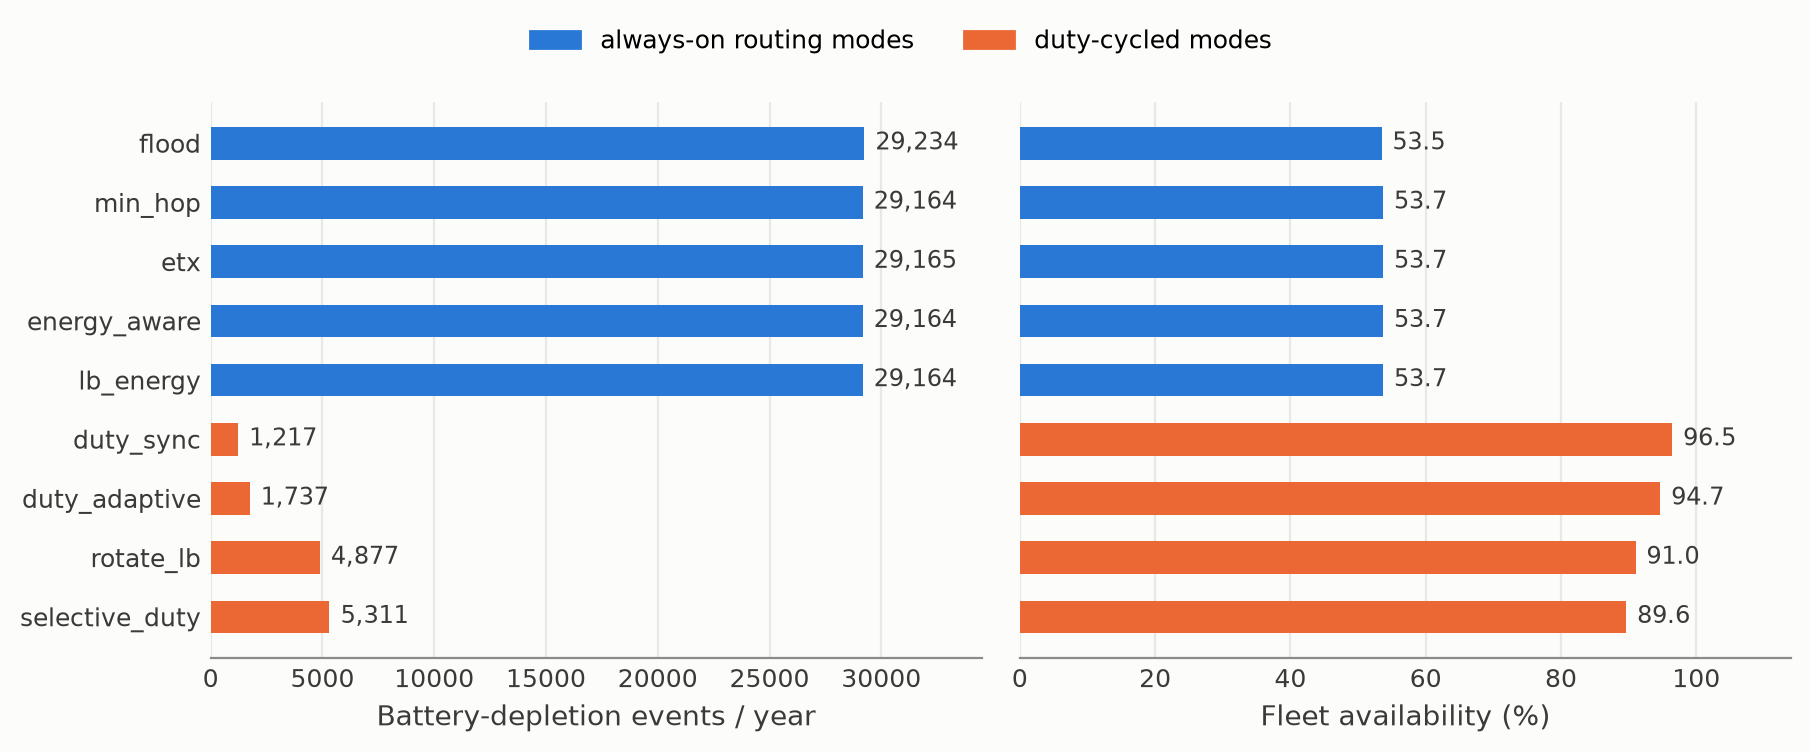
\includegraphics[width=\textwidth]{figures/mode_survivability_tradeoff.png}
\caption{Year-scale survivability by mode (\modelonly, uncalibrated; 9 modes
$\times$ seeds 42--46, 365 days). Left: annual battery-depletion events ---
the five always-on routing modes are indistinguishable ($<0.3\%$ spread)
while duty policies cut depletions ${\approx}5.5$--$24\times$. Right: fleet
availability.}
\end{figure}

All PDR 95\% CIs are below $\pm 0.003$ and deaths-per-year CIs are similarly
tight: given a seed the engine is near-deterministic, so the dominant
uncertainty is the uncalibrated model, not seed noise. Raw counts hid two
things: (a)~always-on modes leave ${\sim}46\%$ of solar fleet-time dark ---
118 of 159 solar sites are available $<$90\% of the year; (b)~uniform
duty\_sync's 94.7\% SOS delivery conceals a 35-minute p95 latency, while
backbone-awake duty modes hold 33--62\,s p95 at 99.3--99.5\% delivery. Every
mode retains rare 1--2\,h worst-case SOS incidents (retry-ceiling limit).
\textbf{No overall winner is declared}: delivery, availability, and SOS tail
latency still trade off, statewide two-engine parity is pending, and the
model is uncalibrated.

\subsection{Central insight: duty policy dominates survivability, not routing}\label{sec:insight}

The five always-on modes span materially different routing strategies, yet
their annual depletion events sit within a \textbf{0.3\% band}
(29{,}164--29{,}234/yr), and four of five share identical availability
(53.7\%) and dark-site counts (118). Switching the \emph{duty/wake policy}
while holding the routing family fixed moves deaths by
$\boldsymbol{\approx 5.5}$--$\boldsymbol{24\times}$ (to 1{,}217--5{,}311/yr)
and fleet availability from ${\sim}54\%$ to 90--96\%. The energy budget is
dominated by idle listening (68\,mA modeled listen vs 12\,mA sleep); what a
node does while \emph{not} forwarding matters far more to survival than
which tree its packets follow. If this survives calibration, solar relay
hardware and firmware should be selected around the wake/CAD architecture,
with routing sophistication a second-order optimization. The quantified cost
--- PDR $-0.05$ to $-0.14$ vs the routed always-on modes ($-0.10$ to $-0.18$
vs flood) plus the SOS-latency structure above --- makes this an explicit,
tunable trade, not a free win. The separation is bound to release\_v1 pending regeneration (\S\ref{sec:limits}); the concrete reason it is unlikely to be an engine artifact is scale --- the 5.5--24$\times$ effect dwarfs the worst cross-engine discrepancy observed on the repaired engine ($\leq 1.3\%$, \S\ref{sec:xval}). (\modelonly; the listen/sleep currents are
bench-calibration placeholders --- precisely why the bench test and a
controlled field day are the critical path.)

\section{Trial 2: the field campaign}\label{sec:trial2}

\textbf{The causal frame, stated plainly: the two-radio controlled-beacon
protocol could not be executed because the beacon node's hardware failed
during the field week --- its internal battery would not hold charge, and its
USB-C charging port then broke. Trial~2 was therefore adjusted --- with every
adjustment registered before the data it affected was collected --- to a
receiver-only field day scoring prospective public-station contact
predictions. The controlled-beacon prediction packs remain frozen and
unscored for a future two-radio day.}

\subsection{Preregistration and freezes}

The strongest freeze in the record is the 2026-07-19 preregistration
(\path{artifacts/trial2/prereg_manifest.json}): 12 hashed inputs ---
prediction tables, generator, DEM manifest, radio metadata, eligibility gate,
analysis code --- bound at git \code{3d15a57} with a clean worktree, before
any calibration-eligible data existed. (Disclosure: 22 rig-bringup telemetry
rows tagged \code{trial2-moosilauke-20260719}, containing no beacon packets,
predate the freeze timestamp by minutes.) The field-day prediction pack for
Moosilauke/Kearsarge/Monadnock is registered via SHA-256 digests recorded in
dated siting documents (2026-07-23; CSV \code{a85e4d08\ldots}, manifest
\code{3e6df03f\ldots}), re-verified matching on 2026-07-26; these registrations were git-timestamped by commit \code{1229309} on 2026-07-26.

\subsection{Campaign log: attempts 1--3 (Jul 18--21)}

Sat Jul~18: the rig never ran (0 GPS, 0 telemetry rows). Sun Jul~19
(Moosilauke): preserved GPS and telemetry evidence covers 09:10--10:19 EDT (${\approx}1.1$\,h; 35{,}891 NMEA sentences), with the receiver radio's serial live only 09:14--10:13 EDT; \textbf{zero beacon packets --- the beacon
was already broken}. Tue Jul~21 (retry): GPS logged throughout the ${\approx}3$-hour attempt (13:21--16:23 UTC, 110{,}115 sentences); the radio never enumerated on USB (power-only cable; 0 radio rows). All raw evidence is
preserved in \path{artifacts/trial2/raw_pull_20260721/} (\code{telemetry\_stream.jsonl}: 65{,}271 lines, 65{,}268 parseable JSON rows; \code{nmea\_stream.jsonl}: 190{,}680 lines; SHA256SUMS added 2026-07-26). Per the frozen
protocol's own definition these are operational failures with preserved evidence.

\subsection{The siting-decision basis and the re-siting criterion}

With the beacon dead, the only possible RF sources were public Meshtastic
stations, so the field day had to sit inside the live public-mesh region. A
checksummed snapshot of the regional community's live dashboard (2026-07-23,
\path{artifacts/trial2/nhmesh_live_snapshot_20260723/}) showed the ecosystem
had largely migrated to a different protocol: \textbf{544 of 550
recently-positioned nodes were MeshCore --- a protocol Meshtastic radios
cannot receive --- leaving 6 Meshtastic stations on the map, none in the
White Mountains} (point-in-time caveat, stated plainly: this was a collector-view snapshot, not an ecosystem census --- a same-dashboard pull on 2026-07-26 12:20 UTC, archived at \path{artifacts/trial2/nhmesh_activity_20260726/}, shows 276 positioned Meshtastic nodes seen within 12\,h; the 2026-07-23 snapshot is preserved because it is what the siting decision was made on). ITM feasibility ranking over the statewide DEM
selected Mt.~Monadnock, then --- when a site policy constraint ruled
Monadnock State Park out --- Pack Monadnock (Miller State Park). Both
sitings were registered in dated documents before their field days.

\subsection{Monadnock: registered, never executed}

The Monadnock pack (beacon point $42.86010/-72.10682$ at 909\,m by the
${\geq}850$\,m first-ascent rule; 33 route samples; 8 prediction rows
appended with prior sites verified byte-identical; DEM sha
\code{57936e6b\ldots}; contact predictions
\path{monadnock_livemesh_predictions_20260723.json}, sha
\code{aba23c13\ldots}) was fully registered on 2026-07-23 and never walked.
It stands as a frozen sibling registration.

\subsection{Pack Monadnock (2026-07-26): the first operationally successful day}\label{sec:packday}

Executed under \code{trial2-packmonadnock-20260726} on the OSM-routed Wapack
loop. The rig ran end-to-end: radio logging all day, 1\,Hz GPS, summit reached (714.6\,m raw GGA maximum, 13:50:13 UTC) with a 13:31--14:04 UTC dwell
within 60 vertical meters of the maximum. Raw evidence:
\path{artifacts/trial2/raw_pull_20260726/} with SHA256SUMS. Trial-ID bookkeeping is disclosed in full: the rig was powered at home from 10:01 UTC; 8 field-day boot rows (10:01--10:06 UTC) plus 55 rows from a 2026-07-22 bench session carry the superseded \code{trial2-moosilauke-20260722} tag (the field tag activates at 10:07:38 UTC); 27 pre-departure rows and 8 post-hike drive-tail rows carry the field tag.

Radio operation, all field days: stock FCC-certified consumer hardware
(Heltec~V3 receiver), unmodified firmware and transmit power, standard US
915\,MHz ISM-band frequencies (LongFast defaults), default channel-access
behavior, the default public channel carrying the project's own traffic, all
equipment placed and retrieved the same day.

\textbf{Registered contact predictions and outcomes --- scored in two
provenance tiers, never aggregated} (the receiver's decode capability is
independently evidenced: it logged foreign frames during the campaign,
including one during the summit dwell at $-117$\,dBm):

\begin{description}
\item[Tier 1 --- pre-departure registered pack]
(\path{packmonadnock_livemesh_predictions_20260726.json}, sha
\code{71db9f00\ldots e9e2}; recorded pre-collection in the siting document in
truncated form, full digest in its addendum): Greenville,
\textsc{contact\_predicted} at $-87.9$\,dBm best-along-route --- \textbf{not
heard (0/1)}. Keene Court St, \textsc{no\_contact\_predicted} at
$-144.4$\,dBm --- \textbf{null held (1/1)}. Three \textsc{marginal} links ---
none heard.
\item[Tier 2 --- trailhead supplement]
(\path{packmonadnock_livemesh_supplement_20260726.json}, sha
\code{f50bda83\ldots 53c5f}; provenance explicitly weaker: digest first
durably recorded post-collection, pre-walk timestamp self-asserted): three
additional \textsc{contact\_predicted} links ($-90.2$ to $-91.1$\,dBm) ---
none heard; four
additional predicted nulls --- all held.
\end{description}

Null confirmations are scored but carry little evidential weight: the same
transmit censoring that voids the contact misses (\S\ref{sec:fieldfindings})
applies symmetrically --- a station that does not transmit produces a held
null regardless of link physics --- and the Keene prediction ($-144.4$\,dBm)
lies ${\approx}13$\,dB below the assumed decode floor, making its null
near-trivial.

\subsection{Field findings: the empirical case for the controlled beacon}\label{sec:fieldfindings}

The contact misses are \textbf{transmit-censored, and the campaign measured
the censoring}:

\begin{enumerate}
\item \textbf{Transmit-opportunity starvation.} The public stations' measured transmit cadence (60-minute activity window generated 2026-07-26 15:02:52 UTC; archived with checksums at \path{artifacts/trial2/nhmesh_activity_20260726/}; an adjacent-hour estimate, ${\approx}$14:03--15:03 UTC, assumed representative of the dwell window) is 0--4 packets per hour per station --- Greenville sent 1 packet in the archived hour, i.e.\ ${\approx}0.6$ expected transmissions during the 33-minute GPS-verified summit dwell (13:31--14:04 UTC); two of the three Tier-2 \textsc{contact}-predicted stations sent 0. (A scoreable opportunity $=$ a station transmission while the receiver sits inside that link's predicted-contact route segment.) The receiving side was equally starved in reverse: the project node
kept stock broadcast cadence and was never heard by any community collector
all day. A link prediction cannot be confirmed by a station that does not
transmit during the window --- at these cadences the expected number of
scoreable opportunities per field day is approximately zero, regardless of
link quality.
\item \textbf{Hop ambiguity.} All six origin-decoded foreign frames logged across the day carry \code{hops\_away} between 1 and 5 (or undecodable hop fields) --- \textbf{zero direct receptions among origin-decoded frames} (one additional frame with undecodable origin carries \code{hops\_away=0}; disclosed, not scored). Mesh-relayed packets attribute their RSSI to an unknown
last-hop transmitter, not to the origin path, so none of the six decodes is
usable as a path-loss observation. (Systems observation, reported as such:
packets originating at stations 86--88\,km away reached the project radio through the mesh --- both such decodes logged in the post-hike vehicle segment --- multi-hop delivery functioning in the wild.)
\end{enumerate}

Together these two measurements are the empirical justification for the
frozen protocol's two central rules --- a controlled beacon at 30\,s cadence
(defeats opportunity starvation) and \code{hops\_away == 0} eligibility
(defeats hop ambiguity). Opportunistic validation against a public mesh fails
not on RF physics but on opportunity statistics and attribution; the
controlled two-radio design is necessary, not merely preferable.

\subsection{The remaining step}

Zero calibration-eligible strata exist; the ${\geq}40$-opportunity target was
never reached on any day; the Moosilauke, Kearsarge, and Monadnock beacon
packs remain frozen and unscored. None of this is dropped or relabeled. The
concrete remaining step is small and fully specified: a replacement beacon
board (${\approx}\$25$), the already-frozen protocol, and one two-radio field day (\S\ref{sec:future}). The raw-dataset package item was built 2026-07-26: \path{artifacts/dataset_release/evidence-2026-07-26/} --- 128{,}721 observations, 0 calibration-grade, with \code{MANIFEST.json} and data dictionary.

\section{Limitations}\label{sec:limits}

\paragraph{Empirical (the binding constraint).} No controlled dataset exists;
Trial~1 and the Trial~2 campaign together yield zero calibration-grade
observations, so the project has no held-out field estimate of RSSI error,
PDR error, or shadow variance. Receiver sensitivity ($-131$\,dBm),
feed/body/foliage losses, board currents, cold-battery capacity, and panel
yield are assumptions or placeholders. Public-mesh observations are
non-calibration-grade by construction (unknown station EIRP/antennas/uptime)
and are never used as path-loss data. A future controlled field day
calibrates propagation and direct-link PDR on its sampled routes; it cannot
by itself validate statewide traffic, routing, kiosk, or annual energy
behavior. Field sites are restricted: one shakedown (Mt.~Washington) and one
operationally successful receiver-only day (Pack Monadnock), summer only.

\paragraph{Modeling.} ITM q50 medians without a validated residual model; q90
route arrays absent. $\sigma = 8$\,dB shadowing, 2\,dB fast fade, capture
threshold, mobile--mobile heuristic, synthetic traffic/SOS rates, and the
600\,s TTL are assumptions. The MAC is not stock Meshtastic firmware. One
statewide weather series; simplified solar geometry; geology priors in the
repository are uncited placeholders not wired into any prediction and are not
model inputs here. The purpose-built simulator is not independently validated
through a widely used third-party framework (ns-3 spot-validation is future
work).

\paragraph{Software, release, and provenance.} Statewide two-engine parity is
pending; corrected-labeled artifacts outside \path{release_v1/} are stale and
marked accordingly. release\_v1 was generated 2026-07-14 from a dirty
worktree (its manifest records this) and carries a disclosed manifest
inconsistency (git \code{d37172c} vs \code{f5e83f0}; the four locked input
hashes agree in both); regeneration (release\_v2) is incomplete (5 of 9
modes, no manifest) and \textbf{not citable} --- the \S\ref{sec:yearscale}
numbers are bound to the archived release\_v1 artifacts. Post-2026-07-19 Trial~2 registrations were committed 2026-07-26 (\code{1229309}); their pre-commit provenance was in-doc SHA-256 digests, as disclosed in the claim-policy note. Authorization for a production fixed-relay deployment
remains an open question (\path{docs/fcc-part15-compliance-memo.md});
field-day operation used certified consumer hardware as marketed
(\S\ref{sec:packday}). Passing tests bound, but do not prove, the absence of
defects.

\section{Future work}\label{sec:future}

(1)~\textbf{The two-radio field day} (the critical path): replacement beacon
board (${\approx}\$25$), the already-frozen protocol (30\,s cadence, sequence
numbers, \code{hops\_away == 0}, ${\geq}40$ opportunities per primary
stratum), scoring the frozen Moosilauke and/or Monadnock packs; the output
feeds the original validation deliverable (RMSE/MAE, predictive-vs-actual
heatmaps, failure matrix) --- all tooling exists. (2)~Bench calibration of
the \textsc{bench-calibrate} constants. (3)~Complete release\_v2 with a full
manifest and regenerate \S\ref{sec:yearscale} from it. (4)~Statewide
two-engine parity per the preregistered tolerance plan. (5)~ns-3
spot-validation of selected MAC/protocol scenarios. (6)~Advisor-decided
amendments: the RSRP$\to$ESP substitution and the ${\geq}40$-opportunity
rule. (7)~Dataset-release packaging: completed 2026-07-26 (\path{artifacts/dataset_release/evidence-2026-07-26/}).

\section{Data and reproducibility statement}\label{sec:repro}

All quantitative statements in this report are artifact-backed measurements,
archived software checks, or simulation results labeled \modelonly. Simulation
numbers cite the corrected multi-seed release (\code{release\_v1},
hash-locked inputs); superseded development-phase outputs are archived
separately in the repository (\path{WITHDRAWN-DO-NOT-CITE/}, with a manifest)
and are not cited here, per the acceptance requirement that superseded numbers
be clearly archived and not mixed with final results. Same-seed engine output
is byte-identical (\S\ref{sec:xval}). Trial~2 registrations made after
2026-07-19 are git-timestamped by commit \code{1229309}; every SHA-256 digest cited in
this report was re-verified against its artifact on 2026-07-26. All artifacts
cited by path in this report resolve in the project repository,
\url{https://github.com/edoherty2017/resilient-emergency-manets-final} (branch \code{main}, release \code{directed-study-final}).

\appendix

\section{Frozen prediction packs and scoring ledger}\label{app:packs}

\begin{table}[h]
\small
\begin{tabularx}{\textwidth}{@{}p{3.4cm}p{4.6cm}X@{}}
\toprule
\textbf{Pack} & \textbf{Registered} & \textbf{Status} \\
\midrule
Mt.~Washington (Ammo/Jewell) & 2026-07-19 freeze, git \code{3d15a57}, clean worktree & Deferred --- never walked; retained \\
Moosilauke (Gorge Brook; beacon 44.01708/$-$71.83777 @1352\,m) & fieldday pack, digests recorded 2026-07-23 & Frozen, unscored (beacon failure); awaits two-radio day \\
Kearsarge (Winslow; beacon 43.38735/$-$71.85970 @771\,m) & same pack & Deferred (ITM predicts no public-mesh contact from site); retained \\
Monadnock (White Dot; beacon 42.86010/$-$72.10682 @909\,m) & pack $+$ livemesh JSON (\code{aba23c13\ldots}), 2026-07-23 & Registered, never executed (site policy); retained \\
Pack Monadnock (Wapack loop) & livemesh JSON (\code{71db9f00\ldots}) pre-departure; supplement (\code{f50bda83\ldots}) weaker tier & \textbf{Executed 2026-07-26.} Tier 1: 0/1 contact, 1/1 null held. Tier 2: 0/3 contacts, 4/4 nulls held. Misses transmit-censored (\S\ref{sec:fieldfindings}); evidence basis: complete Pi instrument log \\
\bottomrule
\end{tabularx}
\end{table}

Propagation method detail for all packs: Longley--Rice ITM q50 point-to-point
over USGS 3DEP DEMs, 26.30\,dBm receiver-power reference (the registration files label this quantity ``EIRP ref'' --- a terminology carry-over in those frozen documents, not a numerical discrepancy; the value is identical), receiver height 1.5\,m, station heights as documented per pack (assumed stock where
unpublished, labeled in the registration files).


\section{Design implications: sensitivity of the survivability result}\label{app:design}

This appendix responds to the advisor's request (2026-07-30) to translate the
idle-listening finding of \S\ref{sec:insight} into engineering terms. All
values are \modelonly{} (uncalibrated constants, \S\ref{sec:limits}); the new
sweeps ran on the current repaired engine against the release\_v1 frozen
inputs (17 runs, 365 days each; hash manifest at
\path{artifacts/sim/appendixB_sweeps/}). The 68\,mA baseline reproduces the
release\_v1 depletion count within 0.04\% (29{,}175 vs.\ 29{,}164 at seed 42),
while its PDR differs modestly (0.843 vs.\ 0.866) reflecting post-release
engine repairs --- comparisons below are therefore made within the sweep.

\paragraph{B.1 --- What listen current makes always-on viable?}
Sweeping the router listen current under always-on energy-aware routing
(stock 37\,Wh battery, 6\,W panel):

\begin{table}[h]
\centering\small
\begin{tabular}{@{}rrrr@{}}
\toprule
Listen current & Depletions/yr & Fleet availability & PDR \\
\midrule
68\,mA (ESP32-class, stock) & 29{,}175 & 53.5\% & 0.843 \\
40\,mA & 13{,}647 & 72.4\% & 0.836 \\
20\,mA & 2{,}824  & 90.6\% & 0.832 \\
10\,mA & \textbf{27} & \textbf{99.8\%} & 0.831 \\
5\,mA  & 0 & 100.0\% & 0.831 \\
2\,mA (nRF52-class) & 0 (3 seeds) & 100.0\% & 0.832 \\
\bottomrule
\end{tabular}
\caption{Listen-current sweep (\modelonly; energy\_aware, seed 42; the 5 and
2\,mA rows verified at seeds 43--44).}
\end{table}

Always-on operation becomes viable at ${\sim}10$\,mA on the stock energy kit,
and at the nRF52-class 2--5\,mA receive currents the modeled fleet loses no
node all year --- while delivery is essentially flat across the sweep. In this
model, sufficiently low listen current dominates every duty-cycling policy on
both axes at once, which quantifies the hardware target: bring the radio's
idle receive path under ${\sim}10$\,mA and the duty-versus-delivery trade of
\S\ref{sec:insight} dissolves. (It also identifies listen current as the
first constant to pin at the bench, and makes the wake-up-receiver direction
a natural follow-on study.)

\paragraph{B.2 --- What capacity reaches 90--95\% availability at stock current?}
Holding 68\,mA and sweeping the energy kit:

\begin{table}[h]
\centering\small
\begin{tabular}{@{}rrrrr@{}}
\toprule
Battery & Panel & Depletions/yr & Fleet availability & PDR \\
\midrule
37\,Wh (stock) & 6\,W (stock) & 29{,}175 & 53.5\% & 0.843 \\
74\,Wh & 6\,W & 14{,}856 & 54.9\% & 0.842 \\
148\,Wh & 6\,W & 6{,}546 & 57.2\% & 0.842 \\
74\,Wh & 12\,W & 9{,}657 & 77.9\% & 0.835 \\
148\,Wh & 12\,W & 4{,}014 & 79.9\% & 0.835 \\
296\,Wh & 12\,W & 1{,}776 & 84.0\% & 0.834 \\
148\,Wh & 24\,W & 1{,}551 & \textbf{94.6\%} & 0.832 \\
296\,Wh & 24\,W & 235 & \textbf{98.5\%} & 0.831 \\
\bottomrule
\end{tabular}
\caption{Battery $\times$ panel sweep at stock 68\,mA listen current
(\modelonly; energy\_aware, seed 42).}
\end{table}

Availability is panel-dominated: at the stock 6\,W panel, even $4\times$
battery moves availability only 53.5\%$\to$57.2\%, because winter harvest ---
not storage --- is binding. Reaching the 90--95\% band at stock listen
current requires roughly $4\times$ battery \emph{and} $4\times$ panel
(148\,Wh\,/\,24\,W $\to$ 94.6\%); $8\times$/$4\times$ reaches 98.5\%. Per
relay, that capacity route is materially more expensive than the
listen-current route of B.1, which reaches higher availability on the stock
kit --- the design lever is the receiver, not the battery.

\paragraph{B.3 --- What duty cycle preserves acceptable SOS latency?}
From the released policy comparison (\S\ref{sec:yearscale}, no new runs): the
threshold is structural rather than a percentage. Uniform low-duty
(duty\_sync, 5\%) buys the largest survivability gain (24$\times$) but
crosses the latency cliff --- 94.7\% SOS delivery with a 35-minute p95,
because deliveries ride the 5-minute retry loop. Backbone-awake policies
(rotate\_lb, selective\_duty), which keep the current routing tree's relays
listening and duty-cycle everyone else, hold SOS p95 at 33--62\,s with
99.3--99.5\% delivery while retaining a 5.5--6$\times$ survivability gain.
Within this model, any deployment with an SOS-latency requirement should
duty-cycle \emph{off-tree} nodes only; uniform duty cycling is a
survivability tool for networks without latency-critical traffic.

\end{document}
